\chapter{Serwer}
\label{chap:server}

    Niniejszy rozdział przedstawia zagadnienia związane z procesem implementacji części serwerowej systemu. 

    \section{Podsystem autoryzacji}


    \section{Podsystem zarządzania}

    	Założeniem tej części procesu implementacyjnego nie było stworzenie skomplikowanej aplikacji umożliwiającej zaawansowaną konfigurację systemu, lecz w pełni funkcjonalnego prototypu na potrzeby demonstracyjne.

    	Podsystem został podzielony na dwie współpracujące ze sobą aplikacje. Warstwową budowę podsystemu zarządzania przedstawia rysunek \ref{fig:mngmt_subs_layers}.

    	\begin{itemize}
    		\item Aplikacja GUI

    			Odpowiada za prezentację danych użytkownikowi, tłumaczenie jego akcji na żądania HTTP i wysyłanie ich do aplikacji API.

    		\item Aplikacja API

    			Udostępnia zasoby dla aplikacji GUI. Odpowiada za odbieranie od niej żądań HTTP, przetwarzanie ich i zwracanie stosownych odpowiedzi. Zawiera większą część logiki biznesowej oraz logikę zarządzania i dostępu do danych.
    	\end{itemize}

        \begin{figure}[]
            \centering
            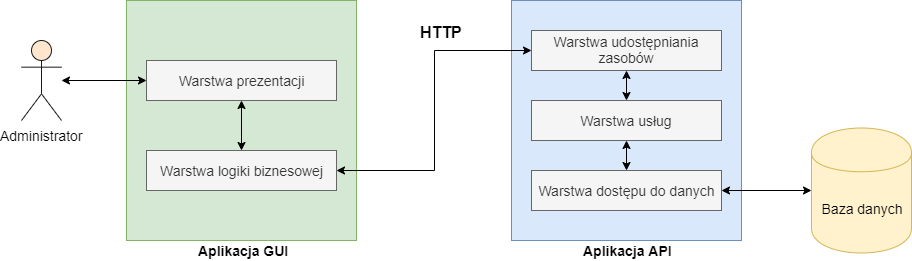
\includegraphics[width=\textwidth]{chapters/images/mngmt_subsystem_layers.png}
            \caption{Warstwowa budowa podsystemu zarządzania}
            \label{fig:mngmt_subs_layers}
        \end{figure}

       	Istotnym czynnikiem motywującym wybór technologii aplikacji podsystemu zarządzania była prostota oraz łatwość implementacji oraz rozwoju funkcjonalnej i estetycznej aplikacji demonstracyjnej zarówno po stronie przeglądarki jak i serwera. Ważną cechą była także łatwość integracji rozwiązania z bazą danych. 

		Do implementacji aplikacji API wybrano język Python z framework'iem Flask. Ważną cechą języka Python jest wbudowane wsparcie dla bazy danych SQLite. SQLite jest biblioteką napisaną w języku C zawierającą implementację niewielkiego silnika bazy danych SQL. Biblioteka języka Python obsługująca silnik umożliwia operowanie na bazach danych umieszczanych bezpośrednio na dysku, co czyni ją rozwiązaniem przydatnym w procesie prototypowania. Framework Flask jest prostą platformą do tworzenia aplikacji internetowych. Dodatkowo zawiera on deweloperski serwer WWW, co znacznie upraszcza proces wytwarzania i testowania aplikacji.

		Do implementacji aplikacji GUI zdecydowano się na framework Angular CLI.

		Wymienione technologie są wystarczające na potrzeby aplikacji prototypowych, jednak w przypadku chęci rozwijania systemu dla środowisk produkcyjnych konieczne mogłoby okazać się przemyślenie zestawu technologii w celu optymalizacji wydajności oraz zwiększenia bezpieczeństwa systemu.